\documentclass[french]{msereport}

\usepackage{listings}

\newcommand{\aws}{\brand{Amazon Web Services}}
\newcommand{\plex}{\brand{PLEX}}

\title{\plex\ in the Cloud with \aws}
\module{CLOUD}{Cloud Computing}
\author{Benjamen Burgy, Jonathan Cornaz}

\begin{document}
	
	\section{Introduction}
		Le but de ce projet est de proposer un déploiement automatisé d’un serveur multimédia privé sur \aws.
		\plex\ (https://plex.tv) est une solution pour la gestion des fichiers multimédias. Il permet (entre autre) de facilement pouvoir naviguer dans sa bibliothèque multimédia et de directement regarder un film ou écouter de la musique. PLEX peut être installé sur n’importe quelle machine et être lié à un support de stockage arbitraire, ce qui permet d’installer chez soi un serveur multimédia privé.
		
		Une des problématiques centrale à résoudre est que \plex\ ne propose pas de système de télé-versement des fichiers. Il a donc fallu développer une petite application web qui permet à l’utilisateur ayant déployé sont serveur multimédia de télé-verser ses fichiers.
	
	\section{Déploiement} 
		Le but est de déployer sur \aws\ trois entités distinctes, à savoir un emplacement pour le stockage de fichier (S3), un serveur de média \plex\ et une petite application web développé par nos soins. Le script doit automatiser un maximum les tâches à effectuer pour simplifier le déploiement à l’utilisateur.
		Il y a cependant des étapes que nous ne pouvons pas automatiser et que l’utilisateur doit effectuer lui-même :
		\begin{itemize}
			\item Créer un compte Amazon Web Service (s’il n’en a pas déjà un)
			\item Créer et télécharger une paire de clé (keypair)
			\item Déposer la clé dans le dossier “deploy”
			\item Créer fichier de config YAML (voir exemple)
			\item Installer les dépendances
			\begin{itemize}
				\item Python et PIP
				\item pip install -r requirements.txt
			\end{itemize}
			\item Exécuter le script de déploiement (python deploy.py \textless config\_file\textgreater )
		\end{itemize}

		Une fois ces opérations effectuée, le script va se charger de créer un espace de stockage, démarrer des machines (une pour \plex\ et une pour le serveur web), configurer les machines pour pointer vers l’espace de stockage et démarrer les services nécessaires.
	
	\section{S3 Storage }
		Le but est d’avoir une zone de stockage centrale des fichiers télé-versés par l’application web et utilisable par le serveur de média \plex. Nous avons donc créée une instance pour un emplacement de stockage S3 (bucket). Cela a été fait via un script afin de pouvoir proposer ce déploiement à des tiers qui n’aurait alors qu’à spécifier le nom de l’emplacement de stockage qu’ils désirent.
		
		Une fois un espace de stockage instancié, il convient de se poser la question de la façon d’y accéder à ces données. En l'occurrence, nous ne pouvions pas modifier PLEX et avons donc choisi de pouvoir “monter” cet espace de stockage comme un système de fichier dans les machines.
		
		Pour y arriver plusieurs solutions existent et nous avons évalué la possibilité d'utiliser s3fs (fuse), s3backer (qui se base sur le précédent) et s3ql. Le problème avec fuse, est qu’il est nécessaire d’obtenir l’intégralité d’un fichier avant de pouvoir l’utiliser. Comme il est question ici d’un serveur de média, cela implique des fichiers volumineux, et il n’est pas envisageable de forcer l’utilisateur à attendre que son film soit complètement téléchargé par le serveur de média avant qu’il puisse le regarder. C’est pourquoi nous avons opté pour s3ql crée un système de fichier qui lui est propre et split les fichiers par bloc de 10 méga-octets. (paramétrable)
	
	\section{Serveur PLEX}		
		Nous avons créé une machine et y avons installé PLEX ainsi que s3ql. Nous avons fait une image de cette machine et l’avons rendu publique (ami-ad8524de) ce qui nous permet de proposé un script qui instancie une machine depuis cette image, sans avoir besoin de diffuser des informations sensibles concernant notre compte \aws.
				
		Comme il n'est pas possible que plusieurs machines montent simultanément le même "bucker" il, faut également le serveur \plex\ partage sont dossier sur le réseau via NFS. Comme ce partage doit être restreint uniquement au serveur web, ceci ne peut se faire qu'au déploiement.
		
		Le script de déploiement se charge donc d’instancier une nouvelle machine sur la base de cette image, d’y envoyer les informations de connexion à l’emplacement de stockage, de monter le stockage dans un dossier (/mnt/s3), de partager ce stockage avec le webserveur (via NFS) et démarrer le service \plex.
	
	\section{Application Web}
		Nous avons développé une petite application dans le but de gérer le stockage des médias de Plex à travers le web. L’application permet des opérations simples dans sa première version comme l’ajout de répertoires et fichiers et leurs suppression. Elle supporte le téléchargement sur le S3 storage de fichiers de grandes tailles.
		L’application utilise le concept de Single Page Application, les librairies \brand{AngularJS}, \brand{Bootstrap} pour la partie client et \brand{Flask} pour la partie serveur en python.
		Elle peut être configuré par le biais d’un fichier settings.yml à la racine du serveur. L’installation de l’application web se fait facilement avec les commandes suivantes:
				
		\code{pip install -r requirements.txt --upgrade \&\& bower install \&\& python index.py}
		
		\begin{figure}[h]
			\label{webserver}
			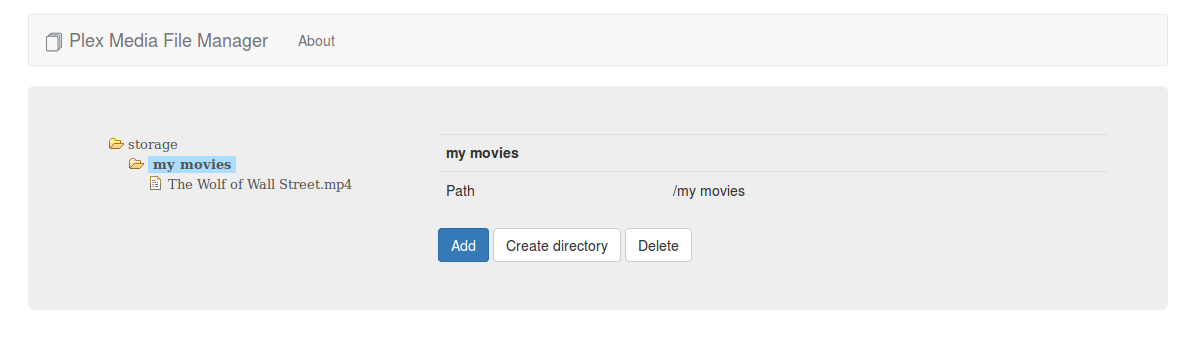
\includegraphics[width=\textwidth]{screen_webserver.png}
			\caption{Application web}
		\end{figure}
		
	
	\section{Conclusion}
		Nous avons pu développer et déployé l'embryon d’une application qui pourrait séduire de nombreux clients désirant un stockage privé sur une infrastructure solide et performante tel que le propose \aws.
		
		Le déploiement utilise les dernières technologies et il est très facile d’installer autant la partie PLEX que la partie web à travers une ligne de commande utilisant Python comme langage de programmation pour l’automatisation.
			
	
	\appendixsection
	
		\listoffigures
		
		\subsection{Sources}
			Les sources sont livrées avec le présent rapport et peuvent être obtenues sur notre repository github: \url{https://github.com/slimaku/hesso.cloud.plex}
		
\end{document}
